\section{Riemannův integrál a jeho aplikace}



\begin{enumerate}
\item Nech je funkia $f(x)$ definovaná na uzavretom intervale $[a,b]$. \\
\begin{enumerate}
\item[I)]{Zavedieme delenie $d$: $a=x_0<x_1<...<x_n=b$.\\
\begin{tikzpicture}[scale=0.6]
\begin{axis}[
    xtick={},ytick={},
    x=4cm, xmax=4.2,ymax=25,ymin=0,xmin=0.8,
    axis lines=middle,
    clip=false,
    domain=1:4,
      axis y line*=left,
      axis x line*=bottom,
      xtick={1,2,3,4},
     ytick=\empty,
        xticklabels={$a=x_0$,$x_1$,$x_2$,$x_3=b$},%<--Here
      axis line style={draw=none},
    ]
\addplot[smooth, thick,domain=1:4]{1+x^2};
\end{axis}
\draw[->] (-0.5,0) -- (15,0) coordinate (x axis) node[below] {$x$};
\draw[->] (0,-0.5) -- (0,6) coordinate (y axis) node[left] {$y$};
\end{tikzpicture}
}
\item[II)]{Na každom intervale $[x_i,x_{i+1}]$ nájdeme $M_i=\sup  \limits _{[x_i,x_{i+1}]}f(x)$ a $m_i=\inf  \limits _{[x_i,x_{i+1}]}f(x)$.\\
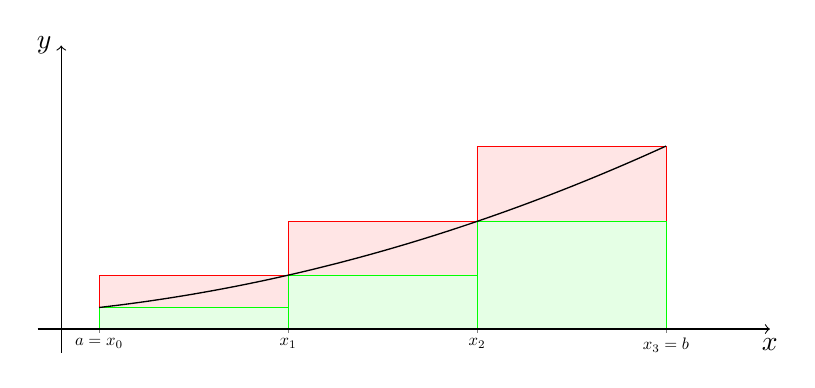
\begin{tikzpicture}[scale=0.6]
\begin{axis}[
    xtick={},ytick={},
    x=4cm, xmax=4.2,ymax=25,ymin=0,xmin=0.8,
    axis lines=middle,
    clip=false,
    domain=1:4,
      axis y line*=left,
      axis x line*=bottom,
      xtick={1,2,3,4},
     ytick=\empty,
        xticklabels={$a=x_0$,$x_1$,$x_2$,$x_3=b$},%<--Here
      axis line style={draw=none},
    ]
    \addplot [draw=red,fill=red!10,const plot mark right, samples=4]
    {1+x^2}\closedcycle;
\addplot [draw=green, fill=green!10, ybar interval, samples=4]
    {1+x^2}\closedcycle;
\addplot[smooth, thick,domain=1:4]{1+x^2};
\end{axis}
\draw[->] (-0.5,0) -- (15,0) coordinate (x axis) node[below] {$x$};
\draw[->] (0,-0.5) -- (0,6) coordinate (y axis) node[left] {$y$};
\end{tikzpicture}
}
\item[III)]{Zavedieme dolný integrálny súčet $s(d)=\sum \limits _{i \in d}m_i(x_{i+1}-x_{i})$ a horný integrálny súčet $S(d)=\sum  \limits _{i \in d}M_i(x_{i+1}-x_{i})$.}
\item[IV)]{Hľadáme dolný Riemannov integrál $\sup  \limits _{d} s(d)=\underline{\int  \limits _{a}^b}f(x)\,dx$ a horný Riemannov integrál $\inf  \limits _{d}S(d)=\overline{\int  \limits _{a}^b}f(x)\,dx$.\\
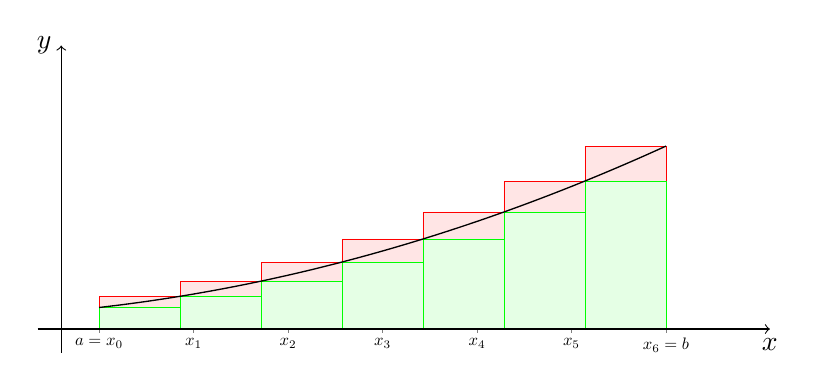
\begin{tikzpicture}[scale=0.6]
\begin{axis}[
    xtick={},ytick={},
    x=4cm, xmax=4.2,ymax=25,ymin=0,xmin=0.8,
    axis lines=middle,
    clip=false,
    domain=1:4,
      axis y line*=left,
      axis x line*=bottom,
      xtick={1,1.5,2,2.5,3,3.5,4},
     ytick=\empty,
        xticklabels={$a=x_0$,$x_1$,$x_2$,$x_3$,$x_4$,$x_5$,$x_6=b$},%<--Here
      axis line style={draw=none},
    ]
    \addplot [draw=red,fill=red!10,const plot mark right, samples=8]
    {1+x^2}\closedcycle;
\addplot [draw=green, fill=green!10, ybar interval, samples=8]
    {1+x^2}\closedcycle;
\addplot[smooth, thick,domain=1:4]{1+x^2};
\end{axis}
\draw[->] (-0.5,0) -- (15,0) coordinate (x axis) node[below] {$x$};
\draw[->] (0,-0.5) -- (0,6) coordinate (y axis) node[left] {$y$};
\end{tikzpicture}
\\
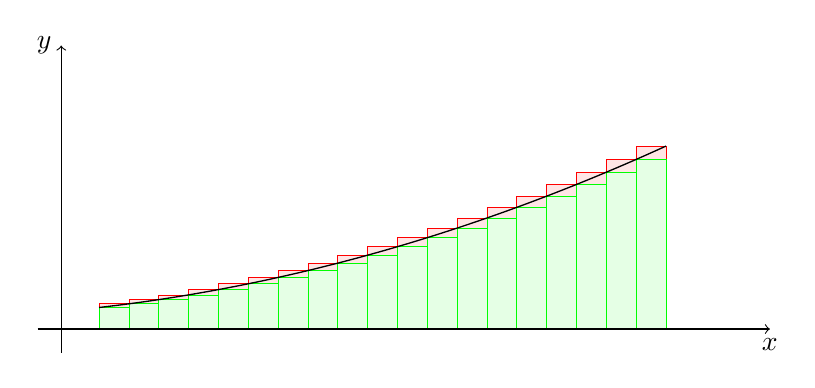
\begin{tikzpicture}[scale=0.6]
\begin{axis}[
    xtick={},ytick={},
    x=4cm, xmax=4.2,ymax=25,ymin=0,xmin=0.8,
    axis lines=middle,
    clip=false,
    domain=1:4,
      axis y line*=left,
      axis x line*=bottom,
     % xtick={1,1.5,2,2.5,3,3.5,4},
     ytick=\empty,
     xtick=\empty,
    %    xticklabels={$a=x_0$,$x_1$,$x_2$,$x_3$,$x_4$,$x_5$,$x_6=b$},%<--Here
      axis line style={draw=none},
    ]
    \addplot [draw=red,fill=red!10,const plot mark right, samples=20]
    {1+x^2}\closedcycle;
\addplot [draw=green, fill=green!10, ybar interval, samples=20]
    {1+x^2}\closedcycle;
\addplot[smooth, thick,domain=1:4]{1+x^2};
\end{axis}
\draw[->] (-0.5,0) -- (15,0) coordinate (x axis) node[below] {$x$};
\draw[->] (0,-0.5) -- (0,6) coordinate (y axis) node[left] {$y$};
\end{tikzpicture}
}
\item[V)]{Pokiaľ sa $\underline{\int_{a}^b}f(x)\,dx=\overline{\int_{a}^b}f(x)\,dx$ funkcia $f(x)$ je integrovateľná na intervale $[a,b]$ a jej \textit{určitý Riemannov integrál} značíme $\int_{a}^bf(x)\,dx$ a jeho hodnota je rovná $\underline{\int_{a}^b}f(x)\,dx=\overline{\int_{a}^b}f(x)\,dx$.\\
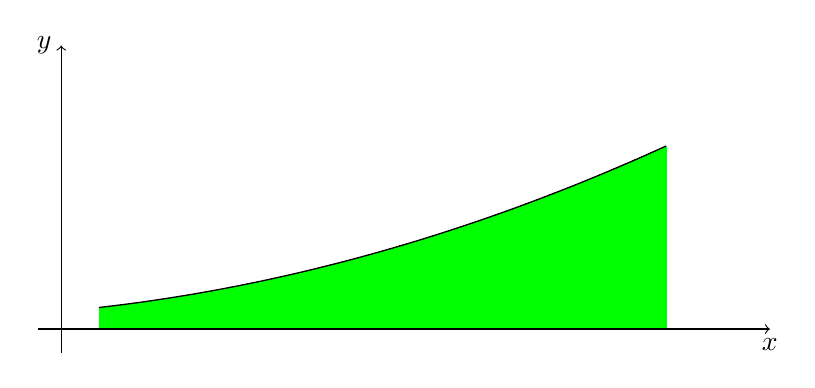
\begin{tikzpicture}[scale=0.6]
\begin{axis}[
    xtick={},ytick={},
    x=4cm, xmax=4.2,ymax=25,ymin=0,xmin=0.8,
    axis lines=middle,
    clip=false,
    domain=1:4,
      axis y line*=left,
      axis x line*=bottom,
     % xtick={1,1.5,2,2.5,3,3.5,4},
     ytick=\empty,
     xtick=\empty,
    %    xticklabels={$a=x_0$,$x_1$,$x_2$,$x_3$,$x_4$,$x_5$,$x_6=b$},%<--Here
      axis line style={draw=none},
    ]
    \addplot [draw=red,fill=red!10,const plot mark right, samples=1000]
    {1+x^2}\closedcycle;
\addplot [draw=green, fill=green!10, ybar interval, samples=1000]
    {1+x^2}\closedcycle;
\addplot[smooth, thick,domain=1:4]{1+x^2};
\end{axis}
\draw[->] (-0.5,0) -- (15,0) coordinate (x axis) node[below] {$x$};
\draw[->] (0,-0.5) -- (0,6) coordinate (y axis) node[left] {$y$};
\end{tikzpicture}}
\end{enumerate}

\item Základné vlastnosti určitého Riemannovho integrálu:
\begin{enumerate}
\item[a)]{\textit{Homogenita}\quad -   $\int \limits_a^b cf(x) \, dx = c \int \limits_a^b f(x) \, dx$, $c \in \mathbb{R}$ pre všetky $c \in \mathbb{R}$ }
\item[b)]{\textit{Aditivita} \quad -  $\int_a^b f(x)+g(x) \, dx = \int \limits_a^b f(x) \, dx+\int \limits_a^b g(x) \,dx$ pre všetky funkcie $f,g$  }
\item[c)]{\textit{Aditivita vzhľadom k definičnému oboru}\quad -   \\$\int \limits_a^b f(x)+g(x) \, dx = \int \limits_a^c f(x) \, dx+\int \limits_c^b f(x) \,dx$, pre všetky $c \in [a,b]$}
\end{enumerate}

\item \textit{Newton-Leibnizova formula}\\
Nech $f(x)$ je spojitá a definovaná funkcia na $[a,b]$. Nech $F(x)$ je primitívna funkcia k $f(x)$. Potom
\begin{align*}
\int \limits_a^b f(x) \, dx = [F(x)]_{x=a}^{x=b}=F(b)-F(a).
\end{align*}

\item Pomocou Newton-Leibnizovej formule vypočítajte určité integrály
\begin{enumerate}

\item[a)]{$\int \limits_0^1x\arctan(x)\,dx$}\hspace{\fill}[$\frac{\pi}{4}-\frac{1}{2}$]
\item[b)]{$\int \limits_1^9\frac{1}{1+\sqrt{x}}\,dx$}\hspace{\fill}[$4-2\ln(2)$]
\item[c)]{$\int \limits_0^{\frac{\pi}{2}}\sin^3(x)\cos^2(x)\,dx$}\hspace{\fill}[$\frac{1}{3}-\frac{1}{5}$]

\item[d)]{$\int \limits_0^1\frac{e^{x}}{1+e^{x}}\,dx$}\hspace{\fill}[$\ln(\frac{1 + e}{2})$]
\item[e)]{$\int \limits_{\frac{\pi}{6}}^{\frac{\pi}{3}}\frac{\sin(2x)}{\cos(x)}\,dx$}\hspace{\fill}[$\sqrt{3} - 1$]
\item[f)]{$\int \limits_0^2 |1-x|\,dx$}\hspace{\fill}[$1$]
\item[g)]{$\int \limits_{-1}^{1}\frac{dx}{x}$}\hspace{\fill}[Nelze použít formule, funkce nesplňuje předpoklady v $x=0$]
\end{enumerate}

\item Vypočítajte obsah obrazcu zadaného pomocou kriviek a načrtnite

\begin{enumerate}
\item[a)]{$y=x^2+2x-3$, os x, $x=0$, $x=3$}\hspace{\fill}[$\frac{37}{3}$]
\item[b)]{$y=-\sin(x)$, $y=0$, $x=\frac{\pi}{3}$, $x=\frac{7 \pi}{6}$}\hspace{\fill}[$\frac{5-\sqrt{3}}{2}$]
\item[c)]{$y=4x^2$, $2x=y^2$}\hspace{\fill}[$\frac{1}{6}$]
\item[d)]{$y=\frac{1}{8}x^3$, $3x-8y+2=0$}\hspace{\fill}[$\frac{11}{32}$]
\item[e)]{$y=x^{-4}$, $x=-1$, $x=-2$}\hspace{\fill}[$\frac{7}{24}$]

\item[f)]{$y=\sin(x), x \in \langle 0;2\pi \rangle$}\hspace{\fill}[$4$]
\item[g)]{$y=\cos(x), y=1-\frac{2x}{\pi}$}\hspace{\fill}[$2-\frac{\pi}{2}$]
\item[h)]{$y=x^2, y^2=x$}\hspace{\fill}[$\frac{1}{3}$]
\item[i)]{$ax=y^2, ay=x^2$, $a>0$}\hspace{\fill}[$\frac{a^2}{3}$]
\item[j)]{$x=a(t-\sin(t)), y=a(1-\cos(t))$, $0 \leq t \leq 2\pi$, $y=0$, $a>0$ (cykloida)}\hspace{\fill}[$3\pi a^2$]
\item[k)]{$x=2t-t^2$, $y=2t^2-t^3$}\hspace{\fill}[$\frac{8}{15}$]
\end{enumerate}

\item Aplikácie určitého integrálu
\begin{center}
\begin{tabular}{|c|c|c|}
    \hline
     & explicitná rovnica &  parametrická rovnica\\
     & $y = f\left(x\right)$, $x\in\left\langle a,b\right\rangle$ & $x=\varphi\left(t\right)$, $y=\psi\left(t\right)$, $t\in\left\langle \alpha,\beta\right\rangle$\\
    \hline 
    PLOŠNÝ OBSAH & $S = \int\limits_{a}^{b}f\left(x\right)dx$ &  $S = \left|\int\limits_{\alpha}^{\beta} \psi\left(t\right)\cdot\dot{\varphi}\left(t\right)dt\right| $\\ \hline
    OBJEM        &$V = \pi\int\limits_{a}^{b}\left[f\left(x\right)\right]^2dx$ & $V = \pi\left|\int\limits_{\alpha}^{\beta} \left[\psi\left(t\right)\right]^2\cdot\dot{\varphi}\left(t\right)dt\right| $ \\\hline
    
    DĹŽKA KŘIVKY & $L = \int\limits_{a}^{b}\sqrt{1+\left[f'\left(x\right)\right]^2}dx$& $L = \int\limits_{\alpha}^{\beta}\sqrt{\left[\dot{\varphi}\left(t\right)\right]^2+\left[\dot{\psi}\left(t\right)\right]^2}dt$\\\hline
    
    POVRCH PLÁŠŤA& $P = 2\pi\int\limits_{a}^{b}f\left(x\right)\sqrt{1+\left[f'\left(x\right)\right]^2}dx $ & $P = 2\pi\int\limits_{\alpha}^{\beta}\psi\left(t\right)\sqrt{\left[\dot{\varphi}\left(t\right)\right]^2+\left[\dot{\psi}\left(t\right)\right]^2}dt$\\ \hline
    \end{tabular}
\end{center}





\item Vypočítajte dĺžku krivky

\begin{enumerate}
\item[a)]Cykloida\\
{$x(t) = a (t - \sin (t))$, $y(t) = a (1 - \cos(t))$}, $a>0, t \in \langle 0;2\pi \rangle$
\hspace{\fill}[$8a$]
\item[b)]{$y=x^{\frac{3}{2}}$, $0 \leq x \leq 4$}\hspace{\fill}[$\frac{8}{27}(10\sqrt{10}-1)$]
\item[c)]{$y^2=5x$, $0 \leq x \leq 3$} (nápověda: integrujte přes osu $y$, poté využijte substituci $y = a\sinh{t}$)
\hspace{\fill}[$2\sqrt{3(3+\frac{5}{2})}$]
\end{enumerate}

\item Vypočítajte povrchy telies
\begin{enumerate}
\item[a)]{vzniknutého rotáciou krivky $y=x\sqrt{\frac{x}{a}}$, $0\leq x \leq a$ okolo osy x}\hspace{\fill}[$\frac{4\pi a^2}{243}(21 \sqrt{13}+2\ln(\frac{3+\sqrt{13}}{2}))$]

\end{enumerate}


\item Vypočítajte objemy těles:
\begin{enumerate}
\item[a)]vzniklého rotací funkce {$y=x^2-2x+5$ kolem osy x, $x \in \langle1;3\rangle$}\hspace{\fill}[$\frac{896\pi}{15}$]
\item[b)]vzniklého rotací jedné periody sinusoidy kolem osy x\hspace{\fill}[$\pi^2$]
\item[c)]vzniklého rotací oblasti ohraničené křivkami {$y=x^2$ a $y=x$ kolem osy x}\hspace{\fill}[$\frac{\pi}{30}$]
\end{enumerate}
\end{enumerate}